\section{Inside FeynCalc}
\label{inside}

This section deals with the internals of \fc. Normal users may be skip it on a first read. For advanced users and people considering contributing to \fc, it is recommended reading.

\subsection{Startup Sequence, Modules, Add-ons and Extensibility}
\label{modules}

\fc is loaded with the following command:

\mcode{<<HighEnergyPhysics`FeynCalc`}

which causes the program file "FeynCalc.m" to be loaded. This file contains definitions of the core objects, used by higher level, functions. Some of the more important of these objects are: \mb{DiracGamma}, \mb{FeynAmpDenominator}, \mb{FourVector}, \mb{LorentzIndex}, \mb{Momentum}, \mb{NonCommutative}, \mb{Pair}, \mb{PartialD}, \mb{PropagatorDenominator}, \mb{QuantumField}, S\mb{UNIndex}, \mb{ScalarProduct}, \mb{Spinor}.

"FeynCalc.m" also scans the subdirectories of the directory "HighEnergyPhysics" for files with an extension ".m". Each such file, like "FeynRule.m", should contain the definition of a function (e.g. \mb{FeynRule}). 

Each definition, whether in one of these files or in "FeynCalc.m" is, however, not loaded into memory. Instead the function name is declared using \mb{DeclarePackage}, so that when this function is used the first time, the definition is loaded into memory. This standard technique significantly reduces startup time and memory consumption. Subdirectories not to be scanned are defined in "FeynCalc.m". The idea is that each directory corresponds to a module, that is, a group of functions pertaining to some subject within quantum field theory. The core modules are:

\begin{itemize}

\item{{\bf \fctables.} Databases of lagrangians, amplitudes and integrals. Important functions: \mb{B0}, \mb{C0}, \mb{Lagrangian}, \mb{Amplitude}, \mb{Integrate2}.}

\item{{\bf \fcloops.} Tools for calculating loop integrals. Important functions: \mb{ OneLoop}, \mb{PaVeReduce}.}

\item{{\bf \fctools.} Various tools for working with quantum fields and amplitudes. Important functions: \mb{Contract}, \mb{DiracReduce}, \mb{FunctionalD}, \mb{FeynRule}, \mb{Tr}, \mb{FermionSpinSum}.}

\item{{\bf \general.} Mathematical tools of a general nature that are used by one or more functions of the other subpackages, but may be useful in other contexts as well.}

\item{{\bf \qcd.} Tools for working with QCD.}

\end{itemize}

The governing idea of the file layout of \fc is modularity. The files belonging to each module are in a separate directory; each file corresponds to one function. If a function uses some support functions or options that are not used by other functions but desirable to have globally accessible, one may put these in the same context as the function and add them to the list \mb{multifunpack} in "FeynCalc.m". Dependence on functions in other contexts should be clearly stated with \mb{MakeContext} statements at the beginning of each file.

The modules listed above all adhere to these conventions.

As will be noticed there are some files and directories not mentioned so far. Apart from the directory "Documentation", which is a directory for standard \mma package documentation, they are listed below under the packages to which they belong. These packages are not loaded by default, but can be enabled by setting certain configuration variables (see section \ref{gamma5}). The reasons for this are: The packages are not considered essential for all users and also don't follow the loading conventions described above and take some time in loading (still of the order of seconds though).

\begin{itemize}

\item{{\bf \fa} is made up of the file "FeynArts.m" , the directories "GraphInfo", "Models" and some more files on the top level of "HighEnergyPhysics". It is an independent package by Sepp Kueblbeck, Hagen Eck and Thomas Hahn for generating Feynman graphs and corresponding amplitudes with Feynman rules as input. Integration within \fc is not intended, but can, with a small effort, be achieved (see \fphi below).
For more information on \fa, see ref \citen{feynarts}.}

\item{{\bf \fphi} is a package by Frederik Orellana providing utilities for working with effective field theories and interacting with \fa. All files belonging to \fphi are contained in the directory "Phi". It was not conceived as a \fc subpackage and the file layout does not adhere to the \fc conventions. Never the less, it has been modified to effectively act as a \fc subpackage and is now distributed only with \fc.}

\item{{\bf \tarcer} is a package by Rolf Mertig for working with 2-loop propagator type integrals. Its file layout also does not adhere to the \fc conventions, but it also is integrated tightly within \fc. The files belonging to \tarcer are contained in the directory "Tarcer". For more information on \tarcer, see ref. \citen{Mertig:1998vk}.}

\item{{\bf \fcdevel} is code which is not considered production ready and is meant to be used by developers only.}

\end{itemize}

\subsection{Configuration and Runtime Variables}
\label{gamma5}

As we have seen, the behaviour of most functions is controlled by options like e.g. \mb{Dimension}. Additionally the behaviour of some functions depends on the setting of certain environment variables. A few of these should be set before loading \fc, namely \mb{\$LoadTARCER, \$LoadPhi, \$LoadFeynArts}.

\otabthree{
{\sl variable name} & {\sl default value} & \cr
\hhline
\mb{\$LoadTARCER} & \mb{False} &  load \tarcer \cr
\mb{\$LoadPhi} & \mb{False} &  load \fphi \cr
\mb{\$LoadFeynArts} & \mb{False} &  load \fa \cr
} {Variables switching loading of extra packages on and off.}

Others can be set at runtime; e.g. \mb{\$Color, \$Covariant, \$Gauge, \$NonComm, \$Abbreviations}. \mb{\$BreitMaison} and \mb{\$Larin} are special in that they are set at runtime, but, once set cannot be changed.

\otabthree{
{\sl variable name} & {\sl default value} & \cr
\hhline
\mb{\$Color} & \mb{False} &  colour special variables \cr
\mb{\$Covariant} & \mb{True} &  display Lorentz indices as upper or lower indices \cr
\mb{\$Gauge} & \mb{1} & the gauge fixing parameter of QED in Lorentz gauge. 1 corresponds to Feynman gauge. Notice that \mb{\$Gauge} is used by some functions, the option \mb{Gauge} by others \cr
\mb{\$NonComm} & \mb{\{DiracGamma, DiracGammaT, 
..., 
% DiracMatrix, DiracSlash, DiracSigma, DiracSpinor, GA, 
% GS, GSD, ChargeConjugationMatrix, RightPartialD, LeftRightPartialD, 
% LeftRightPartialD2, PartialD, QuantumField, SUNT, Spinor, SpinorU, SpinorUBar, SpinorV, SpinorVBar, 
OPESum\}} &  a list of all noncommutative heads \cr
\mb{\$Abbreviations} & \mb{\{"\phat" $\Rule$ "", "*" $\Rule$ "", 
 ..., 
 %"\{" $\Rule$ "", "[" $\Rule$ "", "\}" $\Rule$ "", 
 %"]" $\Rule$ "", "/" $\Rule$ "", "{\bksl}n" $\Rule$ "", "{\bksl}r" $\Rule$ "", " " $\Rule$ "", 
 %", " $\Rule$ "", "AxialVector" $\Rule$ "AV", "Fermion" $\Rule$ "F", 
 %"Momentum" $\Rule$ "", "Pair" $\Rule$ "", "ParticleMass" $\Rule$ "m", 
 %"PseudoScalar" $\Rule$ "PS", "RenormalizationState" $\Rule$ "", 
 %"Scalar" $\Rule$ "S", "SmallVariable" $\Rule$ "sma", "Subscript" $\Rule$ "su", 
"Vector" $\Rule$ "V"\}} &  a list of string substitution rules used when generating names for storing intermediate results. Used by \mb{OneLoop} and \mb{PaVeReduce} \cr
\mb{\$BreitMaison} & \mb{False} & use the Breitenlohner-Maison $\gamma^5$ scheme (currently not supported)\cr
\mb{\$Larin} & \mb{False} & use the Larin-Gorishny-Atkyampo-DelBurgo $\gamma^5$ scheme\cr
\mb{\$VeryVerbose} & \mb{0}& display intermediate messages from \fc \cr
\mb{\$MemoryAvailable} & \mb{8} & the amount of available main memory in megabytes \cr
\mb{\$SpinorMinimal} & \mb{False} & a global switch for an additional simplification attempt in \mb{DiracSimplify} for more than one Spinor line
} {Runtime variables.}

The variable \mb{\$VeryVerbose} may be set to $0, 1, 2$ or 3. 
The higher the setting the more intermediate information is printed during
the calculations.

\fc is designed in such a way that certain intermediate results can be 
stored in order to speed up the computations. 
This of course may  become too memory consuming. 
The storing stops, when the value of \mb{10\phat(-6)*MemoryInUse[\ ]} gets bigger 
than \mb{\$MemoryAvailable-1}.

The default of  \fc is to use the naive $\gamma^{5}$ prescription, i.e.,
$\gamma^{5}$ anticommutes with $D$-dimensional Dirac matrices.
Setting \mb{\$BreitMaison} to \mb{True} changes the commutation behaviour\footnote{
%\mb{DiracTrace}, \mb{DiracSimplify}, \mb{DiracReduce} and \mb{DiracTrick}
In fact, how \fc treats $\gamma^5$ depends on the setting of the variables \mb{\$BreitMaison}, \mb{\$Larin} and \mb{\$West}. They are all boolean variables; the first two specify the $\gamma^5$ scheme. None of them have been neither thoroughly implemented nor tested. If \mb{\$West} is set to True (which is the default), traces involving more than 4 Dirac matrices and a $\gamma^5$ are calculated recursively according to formula (A.5) from \cite{west}, which is based on the Breitenlohner Maison -scheme.
} of $\gamma^{5}$: It anti-commutes with Dirac matrices in four dimensions, 
but commutes with the (D-4)-dimensional part.
The basic features of the Breitenlohner-Maison scheme are implemented in 
\fc, but they have not been tested  very thoroughly (some simple 
calculations are given in  section \ref{diracalg}). 
Therefore one should check the results for correctness.

\subsection{Data Types}
\label{datatypes}

In quantum field theory, a number of types of variables are needed. E.g. variables representing Lorentz indices, momenta, SU($N$) indices and quantum fields. As we have seen in previous sections, the way to tell \fc that a variable is of one of these types is to wrap some head around it. However, \fc provides also a method for having variables be of a certain type without wrapping a head around them. The knowledge about such variables is carried by the function \mb{DataType}. The default setting is

\mcode{DataType[\_\_, \_] := False}

For example, to assign the data-type \mb{PositiveInteger} to the variable \mb{x}, do

\mcode{DataType[x, PositiveInteger] = True}

\otabtwo{\mbs{DataType[{\sl x}, {\sl  type}] = True} & defines the symbol {\sl x} to have data-type {\sl  type} \cr
\mbs{DataType[{\sl x1}, {\sl x2}, ..., {\sl  type}]} & defines the symbols {\sl x1}, {\sl x2}, \ldots to have data-type {\sl  type} \cr}{\fc data-types.}

\otabtwo{
\mbs{NonCommutative} & a variable treated as noncommutative by \mb{Dot}, ``\mb{.}'' \cr
\mbs{PositiveInteger} & a positive integer variable \cr
\mbs{NegativeInteger} &  a negative integer variable \cr
\mbs{PositiveNumber} & a positive number variable \cr
\mbs{FreeIndex} & a Lorentz index not to be contracted by \mb{Contract} \cr
\mbs{GrassmannParity} & \mb{DataType[f, GrassmannParity] = 1} declares a field \mb{f} to be bosonic, \mb{DataType[f, GrassmannParity] = -1} declares it to be fermionic. \cr
}{\fc data-types.}

\beom
\dtog{{DataType[f, g, NonCommutative] = True;\\
}}{}{
Declare some symbols \mb{f} and \mb{g} to be noncommutative.
}
\domtog{{t\ =\ f.g\ -\ g.(2a).f\\
}}{ $f.g\, -\, g.(2a).f$\hfil\\
}{
An algebraic expression using \mb{Dot}, ``.''.
}
\domtog{{DotSimplify[t]\\
}}{ $f.g\, -\, 2a\, g.f$\hfil\\
}{
\mb{DotSimplify} only extracts \mb{a} out of the noncommutative product.
}
\dtog{{DataType[f, g, NonCommutative] = True;\\
}}{}{
Clean up.
}

\dtog{{DataType[m, odd] = DataType[a, even] = True;\\
}}{}{
Declare some symbols \mb{m} and \mb{a} to be of some data-types \mb{even} and \mb{odd}.
}
\dtog{{ptest1[x\_] := x /. (-1)\phat n\_ $\RuleDelayed$ -1 /; DataType[n, odd] ;\\
       ptest2[x\_] := x /. (-1)\phat n\_ $\RuleDelayed$ 1 /; DataType[n, even];\\
}}{}{
Define functions for reducing powers of -1.
}
\domtog{{t = (-1)\phat m + (-1)\phat a + (-1)\phat z\\
}}{ $(-1)^a\, +\, (-1)^m\, +\, (-1)^z$\hfil\\
}{
Redefine the expression \mb{t}.
}
\domtog{{ptest1[t]\\
}}{ $-1\, +\, (-1)^a\, +\, (-1)^z$\hfil\\
}{
Apply the functions to the expression \mb{t}.
}
\domtog{{ptest2[\%]\\
}}{ $(-1)^z$\hfil\\
}{
}
\dtog{{Clear[t];\\
}}{}{
Clear \mb{t}.
}

\enom

\otabtwo{
\mbs{DeclareNonCommutative[{\sl x}, {\sl y}, ...]} & sets \mb{DataType[{\sl x}, NonCommutative] = True; \mb{DataType[{\sl y}, NonCommutative] = True }; ...} \cr}{Declaration of noncommutative variables.}

\subsection{Output Forms and Internal Representation}
\label{int}

%With the default setting of \mb{\$PrePrint\ =\ FeynCalcForm}
By default the internal representation is hidden.
For some purposes, like debugging or hacking the \fc source, however, it may be useful to know how the various objects are represented within \fc.

Some input functions are transformed right away to the internal representation, others only on
being acted upon by utility functions. An example of the first kind is \mb{DiracMatrix[$\mu$]}.
An example of the second kind is \mb{FourVector[p, $\mu$]}; during the internal evaluation of e.g.
\mb{Contract[FourVector[p, $\mu$], FourVector[p, $\mu$]]}, however, a conversion to the internal
representation is done. To see the internal representation of an object, the function
\mb{FeynCalcInternal} can always be used.

The basic idea is to wrap a special head around each special input variable.
For example, the arguments of \mb{MetricTensor[mu, nu]} each get a head 
\mb{LorentzIndex}. These heads have only a few 
functional definitions. A \mb{D}-dimensional \mb{LorentzIndex[mu, D]}, for example, 
simplifies to \mb{LorentzIndex[mu]} when \mb{D} is replaced by 4.

Inside \fc the functions and rules are specified in such a way that they only 
apply to those objects with the right head. 
This programming style, which makes strong use of the pattern matching 
capabilities of \mma, especially the so-called upvalue function definitions, 
has proven to be useful and reliable for the purpose of 
algebraic calculations in physics.

%\otabtwo{
%\mbs{DiracGamma[{\sl x}]} & head of a four-dimensional $\gamma^{\mu}$ or $\ps$ \cr
%\mbs{DiracGamma[{\sl x}, {\sl d}]} & head of a $d$-dimensional $\gamma^{\mu}$ or $\ps$ \cr
%\mbs{LorentzIndex[{\sl mu}]} & head of a four-dimensional Lorentz index $\mu$\cr
%\mbs{LorentzIndex[{\sl mu}, {\sl d}]} & head of a $d$-dimensional Lorentz index $\mu$\cr
%\mbs{Momentum[{\sl p}]} & head of a four-dimensional momentum $p$\cr
%\mbs{Momentum[{\sl p}, {\sl d}]} & head of a $d$-dimensional momentum $p$
%} {Heads of the internal representation.}

\otabtwo{
\mbs{Pair[{\sl a},\ {\sl b}]} &  is a special pairing used in the internal representation: 
{\sl a} and {\sl b} may have heads \mb{LorentzIndex} or \mb{Momentum}. 
If both {\sl a} and {\sl b} have head \mb{LorentzIndex}, the metric tensor is 
understood. If {\sl a} and {\sl b} have head \mb{Momentum}, a scalar product is meant. 
If one of {\sl a} and {\sl b} has head \mb{LorentzIndex} and the other \mb{Momentum}, a Lorentz \
vector (e.g. $p_{\mu}$) is understood \cr
\mbs{Momentum[{\sl p}]} & is a four-dimensional momentum. For other than four dimensions ($d \neq 4 $) use 
\mb{Momentum[{\sl p}, {\sl d}]}. \mb{Momentum[{\sl p}, 4]} simplifies to \mb{Momentum[{\sl p}]} \cr
\mbs{LorentzIndex[$\mu$]} & is a four-dimensional Lorentz index. When $\mu$ is an integer, it evaluates to mb{ExplicitLorentzIndex[$\mu$]}. For other than four dimensions use 
\mb{LorentzIndex[{\sl p}, {\sl d}]}. \mb{LorentzIndex[{\sl p}, 4]} simplifies to \mb{LorentzIndex[{\sl p}]} \cr 
\mbs{ExplicitLorentzIndex[$\mu$]} & is an explicit Lorentz index, i.e., $\mu$ is an integer \cr 
} {Internal representation of Lorentz input functions.}

%In the following it is assumed that \mb{\$PrePrint} has been cleared
%or the default output format type set to \mb{InputForm}, depending on whether
%one is using the terminal or notebook interface.

Now we shall study the internal representation through a few examples. \mb{FeynCalcInternal} shall be applied when necessary.

\beom
%\dtog{{\$PrePrint=.\\
%}}{}{
%Clear \mb{\$PrePrint}.
%}
\dtog{{SetOptions[\$FrontEnd, "CommonDefaultFormatTypes" $\Rule$ {"Output" $\Rule$ StandardForm}];
\\
}}{}{
Suppress \fc typesetting by going from \mb{TraditionalForm} output to
\mb{StandardForm} output. This can also be achieved via the menu setting of
'Cell' $\rightarrow$ 'Default Output Format Type'.
}
\domtog{{DiracMatrix[$\mu$]\\
}}{ DiracGamma[LorentzIndex[$\mu$]]\hfil\\
}{
This is the internal representation of a $\gamma^{\mu}$ in four dimensions.
}
\domtog{{DiracMatrix[$\mu$, Dimension$\Rule$D]\\
}}{ DiracGamma[LorentzIndex[$\mu$, D], D]\hfil\\
}{
Here is a $\gamma^{\mu}$ in $D$ dimensions.
}
\domtog{{DiracSlash[q] . DiracSlash[q, Dimension $\Rule$ D]\\
}}{ DiracGamma[Momentum[q]] . DiracGamma[Momentum[q, D], D]\hfil\\
}{
This is a product of a four-\\
dimensional $\qs$ and 
a $D$-dimensional $\qs$.
}
\domtog{{DiracSimplify[\%]\\
}}{ Pair[Momentum[q], Momentum[q]]\hfil\\
}{
This shows the convention for a four-dimensional scalar product.
}
\domtog{{MetricTensor[$\mu$, $\nu$, Dimension $\Rule$ D]\\
}}{\ Pair[LorentzIndex[$\mu$, D], LorentzIndex[$\nu$, D]]\hfil\\
}{
The head \mb{Pair} is also used for
metric tensors; in this case in  $D$ dimensions.
The dimension is provided as an argument.
}
\domtog{{\% /. D $\Rule$ 4\\
}}{\ Pair[LorentzIndex[$\mu$], LorentzIndex[$\nu$]]\hfil\\
}{
Changing $D$ to 4 recovers the
default for a four-dimensional $g^{\mu \nu}$.
}
\domtog{{FourVector[p, $\mu$]\\
}}{ FourVector[p, $\mu$]\hfil\\
}{
A four-vector does not immediately evaluate to the internal representation.
}
\domtog{{FourVector[p, $\mu$] // FeynCalcInternal\\
}}{ Pair[LorentzIndex[$\mu$], Momentum[p]]\hfil\\
}{
By applying \mb{FeynCalcInternal} we force the internal representation to
be used: A four-vector is also represented as a \mb{Pair} internally.
}
\domtog{{FourVector[p, $\mu$] FourVector[p, $\mu$] // Contract\\
}}{Pair[Momentum[p], Momentum[p]]\hfil\\
}{
By applying some utility function, transformation to the internal representation is
automatically done.
}
\domtog{{FourVector[p, $\mu$, Dimension $\Rule$ D - 4] // FeynCalcInternal\\
}}{Pair[LorentzIndex[$\mu$, -4 + D], Momentum[p, -4 + D]]\hfil\\
}{
A $(D-4)$-dimensional four-vector.
}
\domtog{{\% /. D $\Rule$ 4\\
}}{ 0\hfil\\
}{
It vanishes after changing the dimension to 4.
}
\domtog{{PolarizationVector[k, $\mu$]\\
}}{ Pair[LorentzIndex[$\mu$], Momentum[Polarization[k]]]\hfil\\
}{
Polarization vectors are a special kind of 4-vectors. This shows their internal representation.
}
\enom

\otabtwo{
\mbs{DiracGamma[{\sl x}]} & head of a four-dimensional $\gamma^{\mu}$ or $\ps$ \cr
\mbs{DiracGamma[{\sl x}, {\sl D}]} & head of a $D$-dimensional $\gamma^{\mu}$ or $\ps$ \cr
}{Internal representation of Dirac matrices.}

\otabtwo{
\mbs{Polarization[{\sl k}]} & A polarization vector $\varepsilon(k)$ is understood when the argument of \mb{Momentum} has head \mb{Polarization}\cr
}{Internal representation of Polarization vectors.}

Internally in \fc, all spinors are represented with the same function, \mb{Spinor}. Which of the Dirac spinors $u,v$ and the conjugate spinors $\overline{u}, \overline{v}$ are understood, depends on the position of the spinors in the Dirac chain and the sign of the momentum argument.

\otabtwo{
\mbs{Spinor[{\sl p},\ {\sl m}]} & $u(p,m)$  or  $\overline{u}(p,m)$ \cr
\mbs{Spinor[-{\sl p},{\sl m}]} & $v(p,m)$  or  $\overline{v}(p,m)$ \cr
} {Internal representation of spinors.}

\beom
\domtog{{SpinorV[-p, m] - SpinorU[p, m] // FeynCalcInternal\\
}}{ 0\hfil\\
}{The internal representation of $v(-p,m)$ and $u(p,m)$ is the same.}
\enom

Analogously to Lorentz indices, SU($N$) indices are also wrapped with a head in the internal representation.

\otabtwo{
\mbs{SUNIndex[{\sl i}]} & is an SU($N$) index. When {\sl i} is an integer, it evaluates to ExplicitSUNIndex[{\sl i}]\cr
\mbs{ExplicitSUNIndex[{\sl i}]} & is an explicit SU($N$) index, i.e., {\sl i} is an integer
} {Internal representation of SU($N$) input functions.}

After having completed a calculation with \fc and obtained some screen output, a question will often arise: How does one export the result to a file or to some other application. The screen output in \mb{TraditionalForm} is not very useful; copying and pasting it to a text editor will produce some garbled string with all the typesetting codes of \mma included. Saving an expression with \mb{Put} or \mb{Save} will produce the same as copying the screen output in \mb{InputForm}, namely the internal representation of \fc, which is also not very useful, because it contains all the heads, options, etc. \fc needs to make sense of the expression. For these reasons the \fc external output format exists. An expression in the internal representation is translated to the \fc external output format with the command \mb{FeynCalcExternal}. The inverse translation is done with \mb{FeynCalcInternal}.

Despite the length of the produced output, it can still be useful to see expressions in \mb{InputForm}. To permanently enable this, one can simply evaluate \mb{FI}. What \fc does is setting \mb{\$PrePrint} to \mb{InputForm}. To switch back to typeset output, one can simply evaluate \mb{FC}. Here, \fc clears \mb{\$PrePrint}\footnote{With the terminal interface, \mb{\$PrePrint} gets set to \mb{FeynCalcForm}.}.

\otabtwo{
\mbs{FeynCalcExternal[{\sl exp}]} & translates {\sl exp} from the internal FeynCalc representation to the simpler external one (i.e., \mb{FV}, \mb{GA}, \mb{GS}, etc.) \cr
\mbs{FeynCalcInternal[{\sl exp}]} & translates {\sl exp} into the internal FeynCalc representation \cr
}{Translation to and from external output format.}

\otabtwo{
\mbs{FCE} & just an abbreviation of \mb{FeynCalcExternal} \cr
\mbs{FCI} & just an abbreviation of \mb{FeynCalcInternal} \cr
}{Abbreviation of \mb{FeynCalcExternal} and \mb{FeynCalcInternal}.}

\otabtwo{
\mbs{FI} & disables typesetting of output \cr
\mbs{FC} & enables typesetting of output \cr
}{Switch typesetting off and on.}

\otabthree{
{\sl option name} & {\sl default value} & \cr
\hhline
\mbs{FinalSubstitutions} & \mb{\{\}} & additional translation rules\cr
}{Option of \mb{FeynCalcExternal} and \mb{FeynCalcInternal}.}

\beom
\domtog{{FeynCalcExternal[DiracMatrix[$\mu$], FinalSubstitutions $\Rule \{\mu \Rule mu \}$]\\
}}{ GA[mu]\hfil\\
}{The external output form of $\gamma^\mu$.}
\domtog{{FeynCalcInternal[\%, FinalSubstitutions $\Rule \{mu \Rule \sigma \}$]\\
}}{ DiracGamma[LorentzIndex[$\sigma$]]\hfil\\
}{Translation back to the internal representation.}
\dtog{{SetOptions[\$FrontEnd, "CommonDefaultFormatTypes"$\Rule${"Output" $\Rule$ TraditionalForm}]
\\
}}{}{
Switch back to \fc typesetting by going from \mb{StandardForm} output to
\mb{TraditionalForm} output. This can also be achieved via the menu setting of
'Cell' $\rightarrow$ 'Default Output Format Type'.
}
\enom

\subsection{Help system}

The help system follows standard \mma conventions: Description of an object \mb{obj} is obtained by evaluating \mb{?obj}.

\beom
\domtog{?FeynRule}{ FeynRule[lag, {fields}] gives the Feynman rule corresponding to the field configuration fields of the lagrangian lag.\hfil\\
}{
E.g. the description of the function \mb{FeynRule} is obtained by evaluating \mb{?FeynRule}.
}
\enom

More in-depth information about e.g. \mb{FeynRule} can be obtained by typing in FeynRule in the Add-ons part of the help browser (see figure \ref{help}).

\begin{figure}[ht]
\ifthenelse{\pdf = 0 \or \isundefined{\pdfoutput}}{\setlength\abovecaptionskip{-80pt}}{}
\begin{center}
\scalebox{0.7}{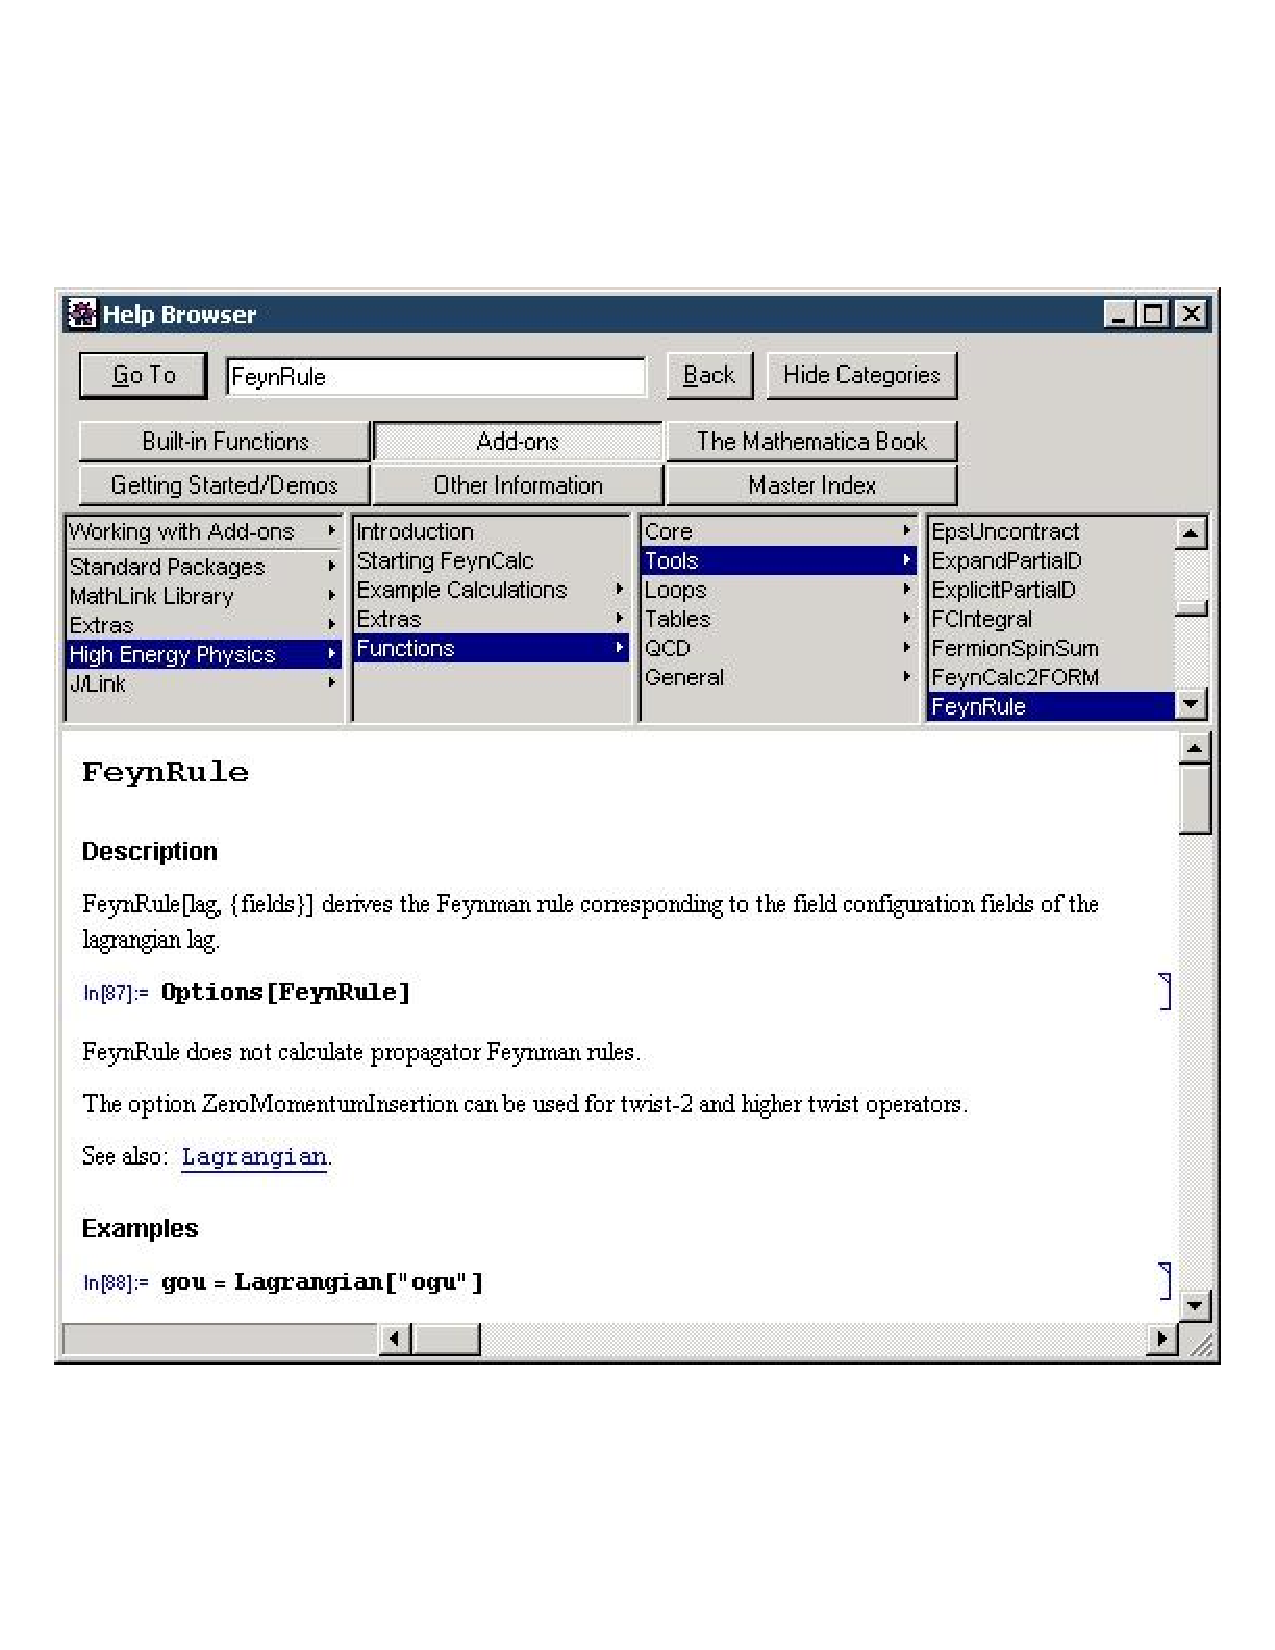
\includegraphics{help}}
\caption{The help system of \fc.}
\label{help}
\end{center}
\end{figure}

The files configuring what appears in the help browser are: "FeynCalcBook.nb" and "BrowserCategories.m" in the directory "HighEnergyPhysics/Documentation/English". The first file is a notebook containing the actual content organized in cells, all of which carry a cell tag. The second file defines the organization of the contents in terms of the cell tags. After a new install of \fc or a change to one of these files 'Rebuild Help Index' from the 'Help' menu must be selected. Then, after clicking the navigation button 'Add-ons' in the help browser window, in the left pane 'High Energy Physics' will appear. Clicking this and the resulting fields in the other three panes will cause \fc help information to appear. The second pane has various introductory material and the field 'Functions'. Clicking this field causes the appearance in the third pane of the fields 'Core', 'Tools', 'Loops', 'Tables', 'QCD' and 'General' corresponding to the file organization of \fc as described in section \ref{modules}. Clicking each of these will display a list of the corresponding objects in the fourth pane. Each of these lists is organized in groups of objects, with the groups in the following order: Functions, abbreviations, constants, options, internal functions. The internal functions are described only for completeness; they are of no interest for other than developers.

